\documentclass{beamer}

% for themes, etc.
\mode<presentation>
%\usetheme{Warsaw}
%\usecolortheme{dolphin}
%{\usetheme{Singapore}}
%{ \usetheme{lined} }
{\usetheme{Dresden}}
\usepackage{fontspec}   %加這個就可以設定字體
\usepackage{xeCJK}       %讓中英文字體分開設置
%\setCJKmainfont{BiauKai} %設定中文為系統上的字型,而英文不去更動,使用原TeX字型
\XeTeXlinebreaklocale "zh"             %這兩行一定要加,中文才能自動換行
\XeTeXlinebreakskip = 0pt plus 1pt     %這兩行一定要加,中文才能自動換行

\usepackage{amsmath,amssymb,amsfonts,booktabs}
\usepackage{epic}
\usepackage{mathpazo}  % fonts are up to you
%\usepackage{astats,epsfig}
\usepackage{graphicx,epsfig,subfigure}
\usepackage{pdftexcmds}
\usepackage{xcolor}
\usepackage{amsthm}
\newtheorem{thm1}{Theorem 1.}
\newtheorem{thm2}{Theorem 2}
\newtheorem{lem1}{Lemma 1.}
\renewcommand{\proofname}{\ctxfk \textbf{Proof.}}
%\usepackage{array,booktabs}
% these will be used later in the title page
\title{Multicollinearity}
\author{San-Teng Huang,Shang-Chien Ho,Hsing-Cheng Pan}
\institute{National Dong Hwa University}
\date{2018/12/19}
\begin{document}
		
		\begin{frame}
		\titlepage
		\end{frame}

\begin{frame}
\frametitle{Outline} % make a frame titled "Outline"
\tableofcontents % show TOC and highlight current section
\end{frame}


\section{Why Collinearity Is a Problem}

\begin{frame}
\frametitle{Multiple Linear Regression}
\emph{•}Consider multiple linear model: 
\begin{equation}
Y_i =  \beta_0 + \beta_1 X_{i1} +\beta_2 X_{i2} +...+\beta_{p-1} X_{ip-1}  + \varepsilon_i \quad , i=1,2,...,n
\end{equation} 
\\\quad where $\boldsymbol{\beta}$ is $p \times 1$ vector, $\mathbf{X}$ is $n \times p$ matrix,
\\\quad and $\varepsilon_i \,\, i.i.d$ with mean $0$, variance $\sigma^2$, for $i=1,...,n$.

\end{frame}


\begin{frame}
\frametitle{Multiple Linear Regression}
\emph{•}The  coefficients of the estimates:
\begin{center}
$\hat{\beta}={\left( X^{T} X\right)}^{-1}X^{T} y$
\end{center}
\emph{•}The variance of the estimates:
\begin{center}
$Var \left[ \hat{\beta}\right] ={\sigma}^2 {\left( X^{T} X\right)}^{-1}$
\end{center}
\quad Even if $X^{T} X$ isn't singular, but is close to being
\\\quad non-invertible, the variances will become huge.
\end{frame}

\begin{frame}
\frametitle{Collinearity}
There are several equivalent conditions for $X^{T} X$,
\\ to be singular or non-invertible:
\\\mbox{}
\\\emph{•}$\det(X^{T} X) = 0$.
\\\emph{•}At least one eigenvalue of $X^{T} X$ is 0. 
\\\emph{•}$X^{T} X$ is rank deficient, meaning that one or more of its columns
\\\quad (or rows) is equal to a linear combination of the other rows.
\end{frame}



\begin{frame}
\frametitle{}
\emph{•}Dealing with Collinearity by Deleting Variables
\\\mbox{}
\\\emph{•}Geometric Perspective
\\\mbox{}
\\\emph{•}Why Multicollinearity Is Harder
\\\mbox{}
\\\emph{•}Diagnosing Collinearity Among Pairs of Variables
\end{frame}

\begin{frame}
\frametitle{}
\begin{figure}[h]
\begin{center}
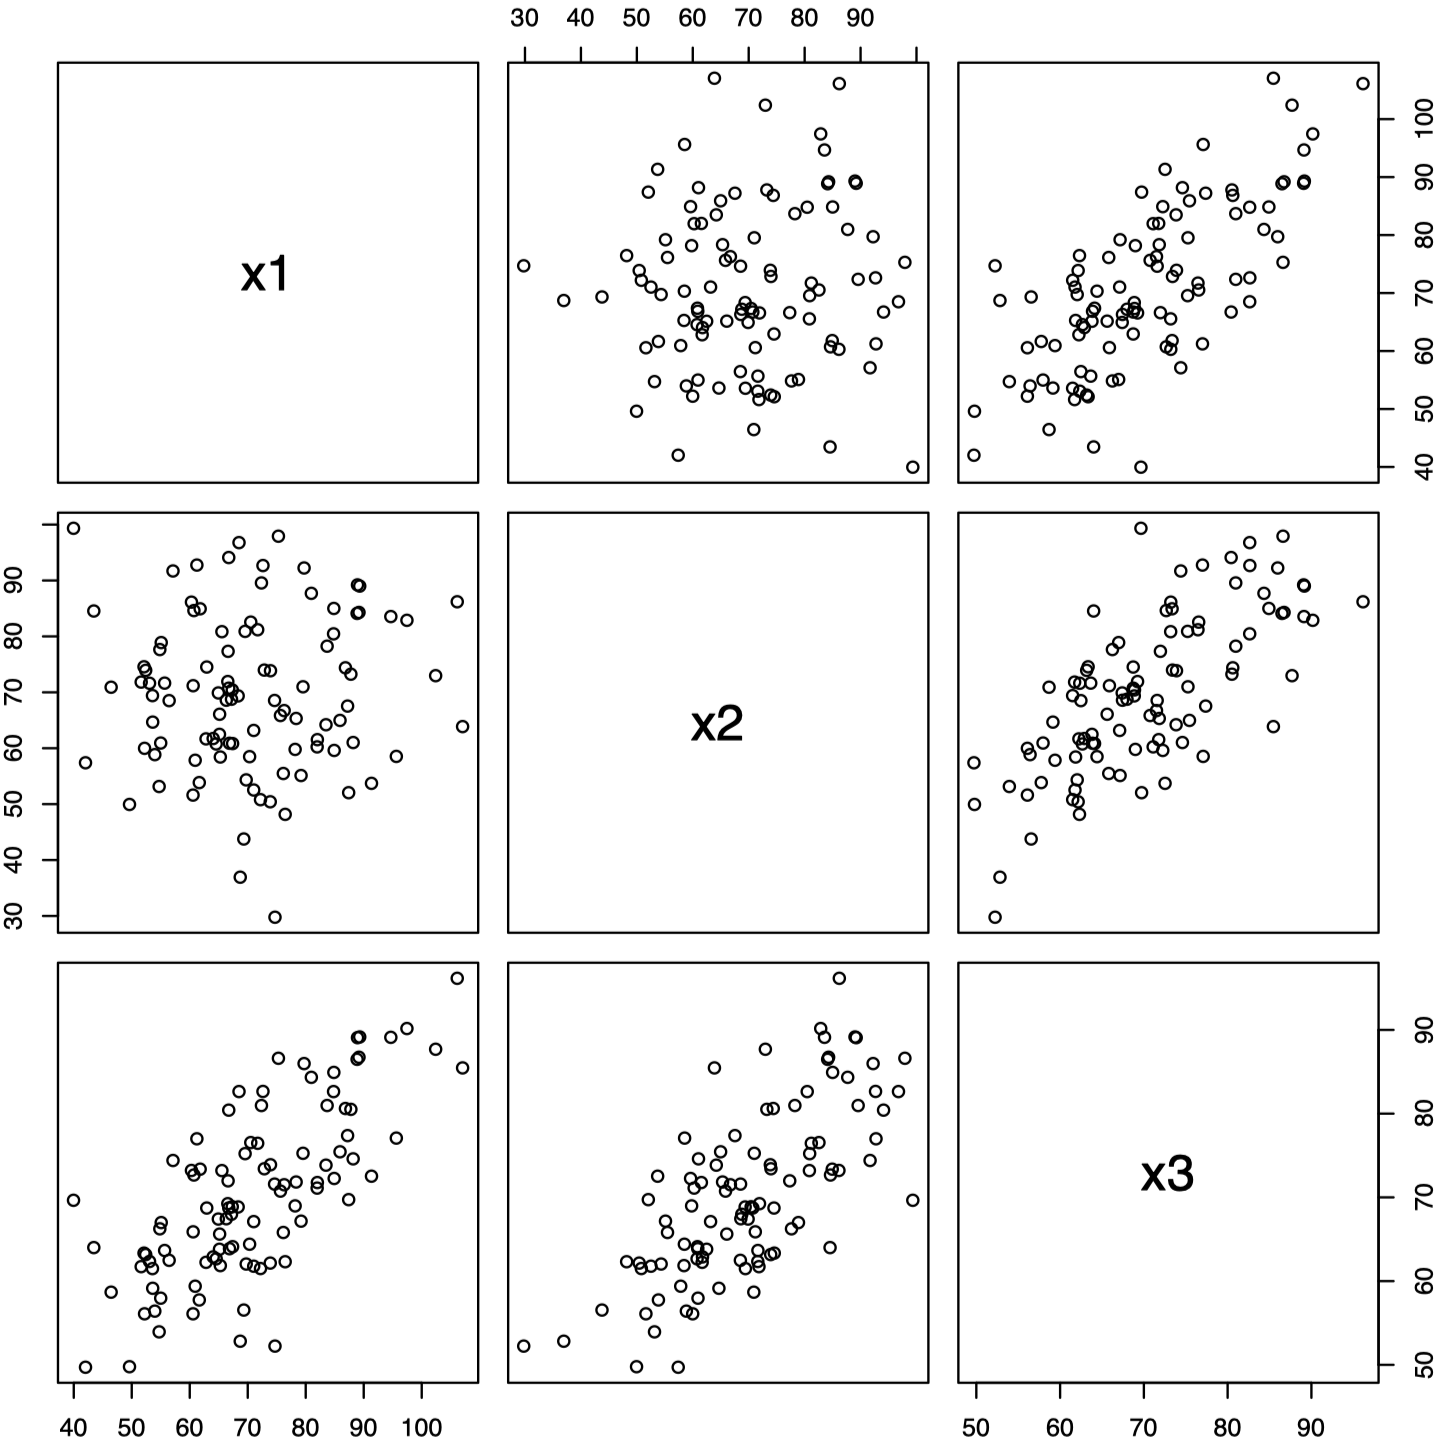
\includegraphics[width=6cm]{image01}
\end{center}
\caption{suppose $X_1$ and $X_2$ are independent Gaussians, of equal variance $\sigma^2$, and $X_3$ is their average,$X_3 = \left( X_1 + X_2 \right)/ 2$}
\end{figure}
\end{frame}


\section{Matrix-Geometric Perspective on Multicollinearity}
\begin{frame}
\frametitle{Multicollinearity}
Multicollinearity means, $\exists \textbf{a} \neq 0 \,\,s.t.$
\begin{equation*}
  a_1X_1+a_2X_2+\hdots + a_pX_p=\sum_{i=1}^{p}a_iX_i=a_0
\end{equation*}
where 
\textbf{a} = $\begin{bmatrix}
a_1
\\a_2
\\\vdots 
\\a_p
\end{bmatrix}$ 
is $p \times 1$ vector, $a_0$ is a constant.
\\That is $\textbf{a}^{T} X = a_0$, for \textbf{a} $ \neq 0$.
\end{frame}

\begin{frame}
\begin{equation*}
\begin{aligned}
Var\left[ \textbf{a}^{T} X\right] &= 0,\quad \textbf{a} \neq 0
\\\mbox{}
\\Var\left[ \textbf{a}^{T} X\right] &= Var\left[ \sum_{i=1}^{p} a_i X_i\right]
\\&=\sum_{i=1}^{p}\sum_{j=1}^{p}a_ia_j Cov\left[ X_i, X_j\right] 
\\&=\textbf{a}^{T} Var\left[ X\right] \textbf{a}
\end{aligned}
\end{equation*}
\end{frame}

\begin{frame}
\emph{•}The eigenvectors of Var[X], such that
\begin{equation*}
Var\left[ X\right] v_i=\lambda v_i
\end{equation*}
\\\emph{•}The eigenvalues are all $≥ 0$.
\\\emph{•}Any vector can be re-written as a sum of eigenvectors:
\begin{equation*}
\textbf{a}=\sum_{i=1}^{p}\left( \textbf{a}^{T} v_i\right) v_i
\end{equation*}
\\\emph{•}The eigenvectors can be chosen so that they all have length 1
\\\quad and are orthogonal to each other.
\\\quad ($||v_i||=1 ,\,and\,\, v_i^T v_j = 0 \,for\, i\neq j$)
%\\\emph{•}Var[X] can be expressed as 
%\begin{equation*}
%Var\left[ X\right] = VDV^{T}
%\end{equation*}
\end{frame}

\begin{frame}
\begin{equation*}
\begin{aligned}
Var\left[ X\right] \textbf{a} &= Var\left[ X\right]\sum_{i=1}^{p}\left( \textbf{a}^{T} v_i\right) v_i
\\&=\sum_{i=1}^{p}\left( \textbf{a}^{T} v_i\right)Var\left[ X\right]v_i
\\&=\sum_{i=1}^{p}\left( \textbf{a}^{T} v_i\right)\lambda_i v_i
\\\textbf{a}^{T} Var\left[ X\right]\textbf{a}  
&= \left( \sum_{i=1}^{p}\left( \textbf{a}^{T} v_i\right)v_j\right) ^{T} \sum_{i=1}^{p}\left( \textbf{a}^{T} v_i\right)\lambda_i v_i
\\&=\sum_{i=1}^{p}\sum_{j=1}^{p}\left( \textbf{a}^{T} v_i\right)\left( \textbf{a}^{T} v_i\right)v_j^{T} v_i\lambda_i
\\&=\sum_{i=1}^{p}\left( \textbf{a}^{T} v_i\right)^2\lambda_i
\end{aligned}
\end{equation*}
\end{frame}
\begin{frame}
\emph{•}The predictors are multi-collinear if and only if Var[X] has  
\\\quad zero eigenvalues.
\\\mbox{}
\\\emph{•}Every multi-collinear combination of the predictors is either 
\\\quad an  eigenvector of Var[X] with zero eigenvalue, or a linear 
\\\quad combination of such eigenvectors.
\end{frame}
	
\section{Eigendecomposition}

\begin{frame}
\frametitle{Finding the Eigendecomposition}
\begin{itemize}
	\item eigen(A) function in R.
	\item numpy.linalg.eig(A) function in Python.
	\item include<Eigen/Eigenvalues> in C++.
	\item eig(A) in matlab.
\end{itemize}
\end{frame}


\begin{frame}
\frametitle{Using the Eigendecomposition}
\begin{enumerate}
\item Find the eigenvalues and eigenvectors. 
\item If any eigenvalues are zero, the data is multicollinear. 
If any are very close to zero, the data is nearly multicollinear. 
\item Examine the corresponding eigenvectors. These indicate the 
linear combinations of variables which equal constants. 
\end{enumerate}
\end{frame}

\begin{frame}
\frametitle{Example}
First make up some data which displays exact multi-collinearity. Let's say that
$X_1$ and $X_2$ are both Gaussian with mean 70 and standard deviation 15, and are
uncorrelated, that $X_3=\frac{(X_1+X_2)}{2}$, and that $Y=0.7X_1+0.3X_2+\epsilon$, with $\epsilon\sim N(0,15)$.
\end{frame}

\begin{frame}
Second input coding below: \\
x1 <- rnorm(100, mean=70, sd=15) \\
x2 <- rnorm(100, mean=70, sd=15)  \\
x3 <- (x1+x2)/2  \\
x4 <- x1+runif(100, min=-100, max=100)  \\
y <- 0.7*x1 + 0.3*x2 + rnorm(100, mean=0, sd=sqrt(15))  \\
df <- data.frame(x1=x1, x2=x2, x3=x3, x4=x4, y=y)  \\
pairs(df)\\
cor(df)
\end{frame}

\begin{frame}
\begin{figure}[h]
\begin{center}
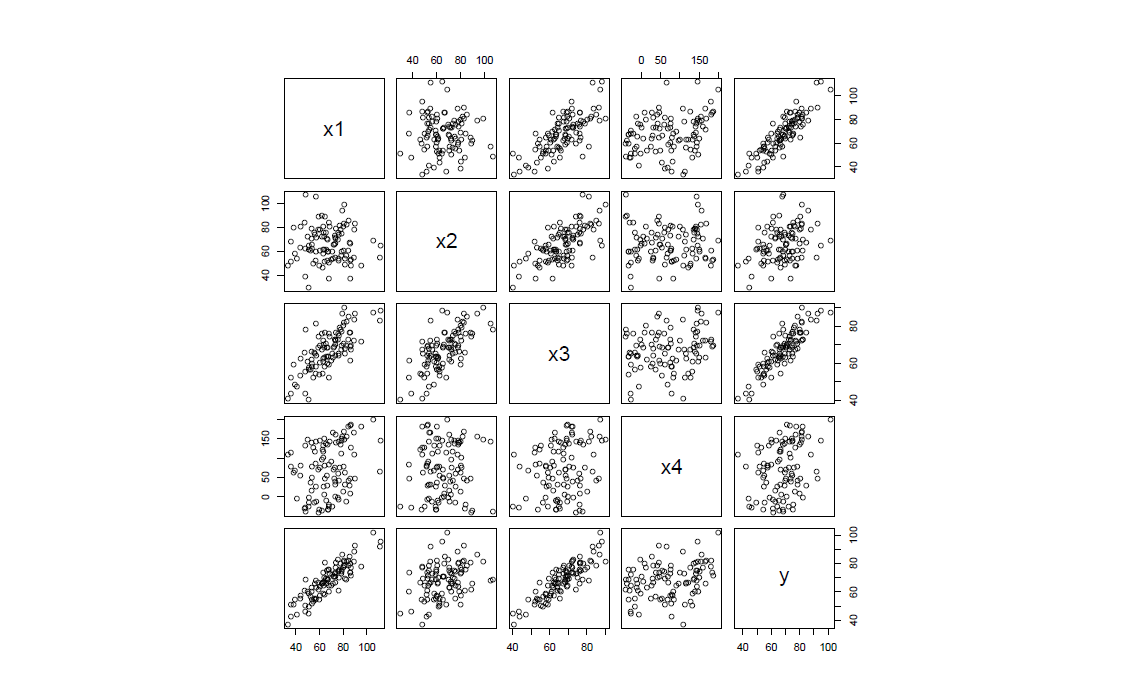
\includegraphics[scale=0.3]{pairsplot}
\end{center}
\end{figure}
\end{frame}

\begin{frame}
\begin{figure}[t]
\begin{center}
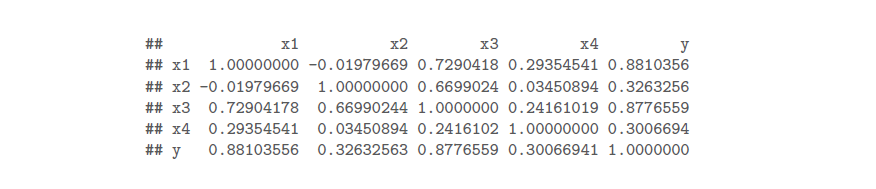
\includegraphics[scale=0.4]{corplot}
\end{center}
\caption{Pairs plot and correlation matrix for the example. Notice that neither the pairs plot nor the correlation matrix reveals a problem, which is because it only arises when considering $X_1$,$X_2$,$X_3$ at once.}
\end{figure}
\end{frame}

\begin{frame}
\begin{figure}[t]

\begin{center}
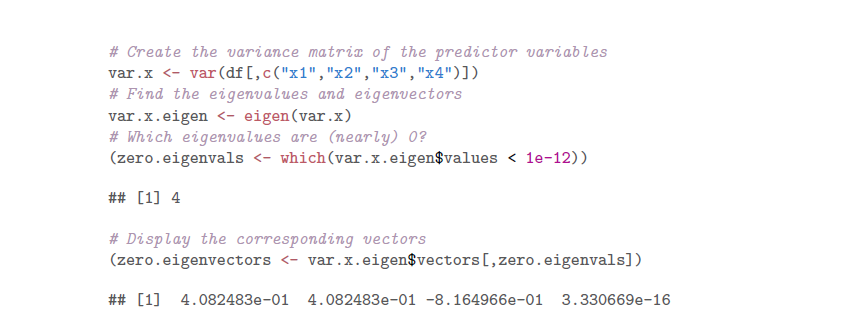
\includegraphics[scale=0.45]{eigenplot}
\end{center}
\caption{\tiny Example of using the eigenvectors of Var[X] to find collinear combinations of the predictor variables. Here, what this suggests is that $-X_1-X_2+2X_3$ = constant. This is correct, since $X3 =\frac{(X_1+X_2)}{2}$, but the eigen-decomposition didn't know this; it discovered it.}
\end{figure}
\end{frame}

\section{Principal Component}
\begin{frame}
\frametitle{Principal Components Regression}
Define new variable:\\
\hspace{1in} $W_1=v_1^{T}X$\\
\hspace{1in} $W_i=v_i^{T}X$\\
\hspace{1in} $W_p=v_p^{T}X$\\
Where $W_1$ is the projection of the original data vector $X$ onto the leading eigenvector, or the \textbf{principal component}. $W_2$ is the projection on the second principal component and uncorrelated with $W_1$. In fact, $\widehat{Cov}[W_i,W_j]=0$ if $i \neq j.$
\end{frame}

\begin{frame}
In \textbf{principal components regression}, we pick some $k \leq p$
$$Y_i = \gamma_{i0}+\gamma_{i1}W_{i1}+...+\gamma_{ik}W_{ik}+\epsilon_i \qquad , i=1,2,3,...,n$$
where $\epsilon$ has expectation 0, constant variance, and no correlation from one observation to another.\\
\end{frame}

\begin{frame}
There are a number of things to be said about principal components regression.
\begin{enumerate}
\item We need some way to pick $k$.
\item The PC regression can be hard to interpret.
\end{enumerate}
\end{frame}

\section{Ridge Regression}

	 
	\begin{frame}
	\frametitle{Ridge Regression}
	\emph{•}The ordinary least squares(OLS) is to
	\begin{equation*}
	  \min\limits_{\boldsymbol{\beta}} (\boldsymbol{Y} - \boldsymbol{X}\boldsymbol{\beta} )^T(\boldsymbol{Y} - \boldsymbol{X}\boldsymbol{\beta} )
	\end{equation*} 
	\emph{•}The ridge regression is to 
	\begin{equation*}
	\min\limits_{\boldsymbol{\beta}} (\boldsymbol{Y} - \boldsymbol{X}\boldsymbol{\beta} )^T(\boldsymbol{Y} - \boldsymbol{X}\boldsymbol{\beta} )  \,\, with \,\, ||\boldsymbol{\beta}||_2^2 \leq c ,\,	 c > 0
	\end{equation*} 
	which is equivalent to 
	\begin{equation*}
	\min\limits_{\boldsymbol{\beta}} (\boldsymbol{Y} - \boldsymbol{X}\boldsymbol{\beta} )^T(\boldsymbol{Y} - \boldsymbol{X}\boldsymbol{\beta} ) + \lambda ||\boldsymbol{\beta}||_2^2 , \, \lambda > 0
	\end{equation*} 
	where $||\boldsymbol{\beta}||_2 = \sqrt{\sum_{j=1}^{p} \beta_j^2 }$.
	\end{frame}

	\begin{frame}
	\frametitle{Geometric Interpretation of Ridge Regression}
	\begin{figure}[h]
	\begin{center}
		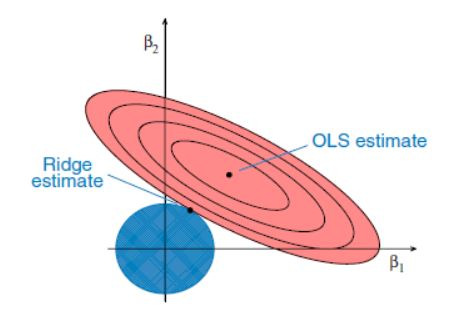
\includegraphics[width=6cm]{image02}
	\end{center}
	\caption{For $p = 2$, the ellipses correspond to the contours of residual sum of squares (SSE), and SSE is minimized at ordinary least square (OLS) estimate.}
	\end{figure}
	\end{frame}

	\begin{frame}
	
	\emph{•}The ridge regression estimator is 
	\begin{equation*}
	\hat{\boldsymbol{\beta}}_{\lambda} = (\boldsymbol{X}^T\boldsymbol{X} + \lambda\boldsymbol{I}) ^{-1} \boldsymbol{X}^T \boldsymbol{Y} 
	\end{equation*}
	where $\lambda > 0$ is a tuning parameter.
	\\\emph{•}Note:
	\\\quad 1. If $\lambda = 0$, then $\hat{\boldsymbol{\beta}}_{\lambda} = (\boldsymbol{X}^T\boldsymbol{X} ) ^{-1} \boldsymbol{X}^T \boldsymbol{Y} $  
	\\\quad 2. If $\lambda \rightarrow \infty$, then $\hat{\boldsymbol{\beta}}_{\lambda} \rightarrow 0$, 
	\\\quad i.e. the larger $\lambda$, the smaller $\beta_j$'s value you will get.
	\\\emph{•}This would break any exact multicollinearity, so the inverse always exists.
	
	\end{frame}
	
	\begin{frame}
	\emph{•}The ridge regression estimator $\hat{\boldsymbol{\beta}}_{\lambda}$ is biased.
	\begin{equation*}
	\begin{aligned}
	E(\hat{\boldsymbol{\beta}}_{\lambda}) & = (\boldsymbol{X}^T\boldsymbol{X} + \lambda\boldsymbol{I}) ^{-1} \boldsymbol{X}^T E(\boldsymbol{Y})
	\\ & = (\boldsymbol{X}^T\boldsymbol{X} + \lambda\boldsymbol{I}) ^{-1} \boldsymbol{X}^T \boldsymbol{X}\boldsymbol{\beta}
	\\Var[\hat{\boldsymbol{\beta}}_{\lambda}] & = Var[(\boldsymbol{X}^T\boldsymbol{X} + \lambda\boldsymbol{I}) ^{-1} \boldsymbol{X}^T \boldsymbol{Y}]
	\\& = Var[(\boldsymbol{X}^T\boldsymbol{X} + \lambda\boldsymbol{I}) ^{-1} \boldsymbol{X}^T \boldsymbol{\varepsilon} ]
	\\& = \sigma^2 (\boldsymbol{X}^T\boldsymbol{X} + \lambda\boldsymbol{I}) ^{-1} \boldsymbol{X}^T   \boldsymbol{X}  (\boldsymbol{X}^T\boldsymbol{X} + \lambda\boldsymbol{I}) ^{-1}
	\end{aligned}
	\end{equation*}
	\emph{•}How to choose the parameter $\lambda$ ?
	\\\quad by using cross-validation.
	\end{frame}

\section{Conclusion}
	
	\begin{frame}
	\frametitle{Problem of High-Dimensional Regression}
 	\emph{•}In high-dimensional data($n < p$), it will always have
 	\\\quad multicollinearity. 
 	\\\quad (since $rank(\boldsymbol{X}) = n < p$ i.e. the column space of $\boldsymbol{X}$ is n, 
 	\\\quad but the number of predictors is p.) \vspace{0.3cm}
 	\\\emph{•}We may 
 	\\\quad (i)reduce the dimension until $< n$.(as in principle components
 	\\\quad regression)
 	\\\quad (ii)penalize the estimates to make them stable and regular.(as
 	\\\quad in ridge regression). 
	\end{frame}

	\begin{frame}
	\frametitle{Conclusion}
	\emph{•}What is multicollinearity ?
	\vspace{0.3cm}
	\\\emph{•}How to deal with multicollinearity ?
	\vspace{0.1cm}
	\\\quad -Pairs Plot of the predictors
	\\\quad -Eigendecomposition
	\\\quad -Principal Components Regression
	\\\quad -Ridge Regression
	\end{frame}

\end{document}        